%*******************************************************************************
% Copyright (c) 2014 Formal Mind GmbH and others
% All rights reserved. This program and the accompanying materials
% are made available under the terms of the Eclipse Public License v1.0
% which accompanies this distribution, and is available at
% http://www.eclipse.org/legal/epl-v10.html
% 
% Contributors:
%     Michael Jastram - initial Copy
%     Maha Jastram - subsequent improvements
%******************************************************************************/

\pror{} has an extension mechanism that allows custom rendering, custom editing and automatic modifications to the requirements model. These extensions are called \term{presentations}.

Presentations can be created and configured via \menu{ProR | Presentation Configuration...} or the icon 
\includegraphics[height=1em]{../rmf-images/icons/full/obj16//ReqIFToolExtension.png} in the toolbar.  Launching it will show the dialog shown in Figure~\ref{fig:presentation-dialog}.  Initially, the dialog will be empty.  The dialog in the figure shows two presentation configurations.

Presentations are specific for a model, and its configuration is also stored in the requirements model.

\pror{} ships with a small set of standard presentations.  Additional presentations can be installed into \pror{}.

\begin{warning}
Note that presentations are specific to \pror{}, not to ReqIF.  This means that other tools will simply ignore presentations.  Also note that the behavior of the tool is unpredictable if a presentation used by a model is not installed in \pror{}.
\end{warning}

\begin{figure}
  \centering
  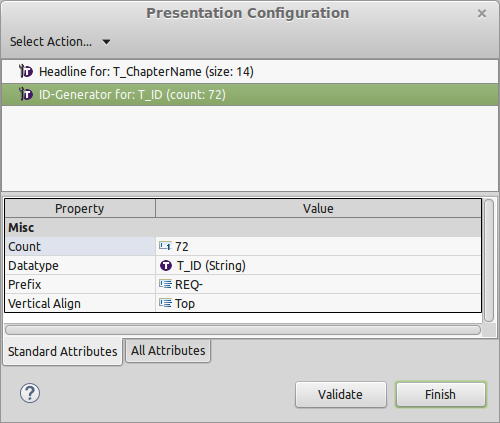
\includegraphics[width=0.8\textwidth]{../rmf-images/presentation-dialog.png}
  \caption{The presentation dialog with two configured presentations}
  \label{fig:presentation-dialog}
\end{figure}

% ===================================================================================
\section{Working with Presentations}
\index{presentation dialog}
% ===================================================================================

All presentations are configured in the same way.  To configure a presentation for the current model, first open the presentation configuration dialog as described above.

Initially, the dialog is empty.  You can add new presentations using the \menu{Select Action...} dropdown.  It will list all built-in and installed presentations.  Upon selecting an entry, it will be added to the list below.

\begin{info}It is possible (and often useful) to add the same presentation multiple times. For instance, one could add multiple ID generation presentations for different types of elements (with correspondingly different prefixes). 
\end{info}

Selecting a presentation in the upper pane will show its configuration parameters in the lower pane.  In Figure~\ref{fig:presentation-dialog}, the ID-Generator is selected, and the lower pane shows its four configuration parameters.

All presentations have a configuration parameter \menu{Datatype}.  Typically, the datatype determines whether a presentation is applied to an element or not.

\begin{info}
  If you want a presentation to be applied to a dedicated \term{Attribute} (rather than \term{Datatype}, then simply create a specific datatype for that attribute. And conversely, you can reuse a single presentation for multiple attributes by using the same datatype for all relevant Attributes.
\end{info}

The order of entries sometimes (but rarely) matters.  Presentations can be reordered using drag and drop.

Last, to delete a presentation, select \menu{Delete} from the context menu by right-clicking.

% ===================================================================================
\section{Default Datatype Handlers}
\index{presentations!default handlers}
\index{default handlers}
% ===================================================================================

Sometimes, it is desirable to use a presentation as the default for rendering (and editing) a specific datatype.  For example, the open source RMF can not render formatted (XHTML) text and instead shows a simplification in plain text.  But \pror{} offers the RTF presentation that allows rich rendering and editing.  Thus, it would be nice if XHTML datatypes would always be rendered using the RTF presentation, if installed.

This is possible.  And in fact, presentations can request to be used as default handlers.  If such a presentation is installed, it will automatically take over from the default.

Users can configure and override this.  To do so, go to \menu{Window | Preferences | ReqIF | Default Presentations}.  The resulting dialog is shown in Figure~\ref{fig:default-handlers}.

\begin{figure}
  \centering
  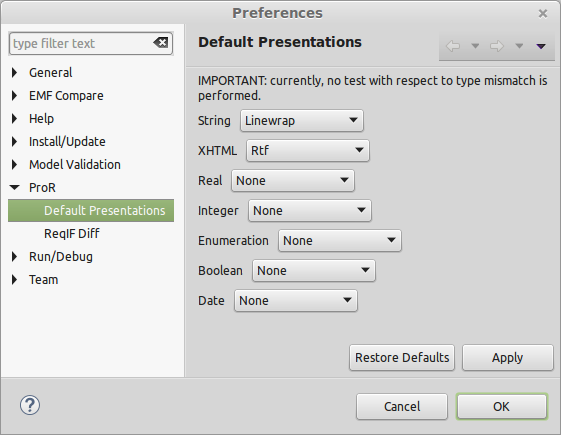
\includegraphics[width=0.8\textwidth]{../rmf-images/default-handlers.png}
  \caption{The preference dialog for handling default presentations}
  \label{fig:default-handlers}
\end{figure}

For each of the standard ReqIF datatypes, a handler can be chosen.  The default is \menu{none}.  The following entries are available:

\begin{description}
\item[None.] This is the default and implies that the build-in renderer is used.   Upon starting the tool, \pror{} will check whether a new presentation has been installed that requests to act as the default handler for that datatype.  If such a presentation is found, it will be set as the handler.
\item[Use Built-in.] This forces the built-in handler to be used.  Even if an installed presentation requests to be the handler, the built-in handler will continue to be used.
\item[List of installed presentations.] The remaining entries list all installed presentations.  Note that the dialog does not filter the matching types.  I.e. even though the RTF presentation is only applicable for XHTML, it is shown in the dropdown for all datatypes.
\end{description}

\begin{warning}
Please make sure that you only set datatype handlers of the correct type.  Also note that there is no access to the configuration parameters of default handlers. Therefore, this mechanism makes only sense for presentations that do not require any additional configuration.
\end{warning}

% ===================================================================================
\section{Built-in Presentations}
\index{presentations!build-in}
% ===================================================================================

The following presentations are part of the Eclipse RMF project and are therefore open source.

% -----------------------------------------------------------------------------------
\subsection{ID Generator Presentation}
\index{presentation!id generator}
\label{sec:id_presentation}
% -----------------------------------------------------------------------------------

This presentation automatically generates user-friendly IDs, consisting of a prefix and a number, e.g. ``REQ-12''. The configuration parameters are shown in Figure~\ref{fig:default-handlers}.

\begin{info}
Attributes to which this presentation applies are read-only and cannot be edited manually any more (as long as the presentation is active).
\end{info}

The parameters are:

\begin{description}
\item[Count.] The counter position. When a new ID is created, it will be incremented by one.  Changing it allows  the user to start or continue with a different number.
\item[Datatype.] The presentation will be applied to all attributes with this datatype.  Must by of type \term{String}.
\item[Prefix.] The prefix to the number.  Note that changing this will only modify newly created IDs, not those already generated.
\item[Vertical align.] Allows to adjust how the text shall be rendered in the cell.
\end{description}

\begin{warning}
Currently, the presentation does not check whether duplicate IDs exist!
\end{warning}

% -----------------------------------------------------------------------------------
\subsection{Headline Presentation}
\index{presentation!headline}
% -----------------------------------------------------------------------------------

This presentation renders the content of a cell boldface in a large font.  This can be useful if
you want to format text to stand out (e.g. a headline), without having to resort to XHTML.

The parameters are:

\begin{description}
\item[Datatype.] The presentation will be applied to all attributes with this datatype.  Must by of type \term{String}.
\item[Size.] The size of the text in point.
\end{description}

% -----------------------------------------------------------------------------------
\subsection{Linewrap}
\index{presentation!linewrap}
% -----------------------------------------------------------------------------------

This presentation wraps text at word boundaries, essentially what one would expect anyway.  The built-in renderer breaks the text anywhere, including in the middle of words.

This presentation is usually set as the default presentation.

\begin{info}
Regular users can just ignore this presentation.  It has been created for developers to understand the presentation mechanism.
\end{info}

